%!TEX root = ../my_thesis.tex
\chapter{Des oscillations du décodage itératif} % (fold)

Dans ce chapitre, on présente le SC et le décodage  à la Benjamin

TODO : osc : rajouter que c'est la même qq soit la taille de trame

\vspace*{\fill}
\minitocTITI
\vspace*{\fill}
\newpage

\section{Introduction}\label{sec:ch2_intro} 
En 1996, Benedetto et Montorsi listent les questions ouvertes liées aux turbo codes \cite{benedetto_unveiling}. La
première, qu'ils qualifient de \og question théorique importante \fg concerne la convergence des algorithmes 
sous-optimaux itératifs. \og Convergent-ils toujours ? Sous quelles conditions ? \fg

Peu après, il a été montré par des arguments géométriques que la convergence de ces algorithmes vers la solution à 
maximum de vraisemblance ou vers une solution stable n'est pas garantie \cite{richardson_geometry}.
Dans \cite{reid_convergence}, l'évolution de la valeur des LLR des informations \textit{a posteriori} est présenté au 
cours des itérations. Les auteurs classifient alors le comportement des LLRs lors du décodage des trames selon 3 modes : 
\begin{enumerate}
	\item Tous les bits convergents rapidement et de la même manière vers une solution stable.
	\item La plus part des bits convergent rapidement vers une solution stable alors que les autres convergent de manière 
	différente (croissance plus lente).
	\item Les valeurs des LLR oscillent, croisant ou non le seuil de décision (0). Dans ce cas, l'allure des LLRs est 
	sinusoïdale.
\end{enumerate}
De ces constatations, les auteurs proposent un critère d'arrêt pour le processus itératif basé sur la valeur moyenne des 
LLRs et d'un seuil. Néanmoins, la valeur du seuil ne peut être déterminé que de manière empirique. %Afin d'améliorer les 
%performances 

D'autres critères d'arrêt basés sur l'analyse des changements de signe des informations produites par les décodeur 
élémentaires avaient déjà été proposés dans la littérature. Le Sign Change Ratio (SCR) \cite{fossorier_scr} est une 
approximation du critère basé sur la Cross Entropy (CE) \cite{hagenauer_ce}. Le principe consiste à compter le nombre de 
changement de signes $C(i)$ des information extrinsèques produites par le second SISO entre l'itération $i$ et $i-1$. 
Des simulations montrent qu'arrêter les itérations lorsque $C(i)\leq (0,0005 \sim 0.03)\times K$ permet d'obtenir les 
mêmes performances en termes de nombre d'itérations moyen utilisées et de décodage que le critère CE.

Le critère d'arrêt nommé Sign Difference Ratio (SDR) \cite{fossorier_scr} est une variante du SCR. Dans ce cas, $C(i)$ 
compte le nombre de fois où l'information \textit{a posteriori} et l'information extrinsèque diffèrent à l'itération $i$. 
Ce critère propose les mêmes performances que le SCR tout en permettant de réduire la quantité de stockage nécessaire.

Ainsi, dans le cadre des turbo codes, les oscillations au sein du décodeur ont été étudiées pour mieux comprendre le 
fonctionnement du processus itératif mais aussi pour fournir des critères d'arrêt performants, c'est à dire permettant de 
réduire significativement le nombre d'itération moyen tout en conservant les performances de décodage obtenues avec un 
nombre d'itération fixe maximal.

Dans le cadre des codes LDPC, le processus de décodage est itératif. De même, des phénomènes oscillatoires sont aussi 
observables. Néanmoins dans le cadre des codes LDPC, les équations de parités permettent la détection d'erreurs. Ainsi, 
les oscillations ont été étudiés dans un but d'améliorer des performances de décodage. Deux approches majeures ont été 
considérées. La première approche consiste en une modification de l'algorithme à propagation de croyance (BP) pour le 
décodage des codes LDPC \cite{gounai_bp_osc}. Son principe est le suivant. Si le nouveau LLR extrinsèque (qui correspond 
au calcul des nœuds de variable) change de signe lors de la nouvelle itération, alors la valeur calculée lors de 
l'itération précédente est sommée à la valeur courante. Les auteurs constates des meilleurs performances de décodage en 
comparaison de l'algorithme BP usuel.

La seconde approche, nommée Self-Corrected (SC) \cite{savin_sc}, est une modification de l'algorithme Min-Sum lui même
étant une simplification du BP. Son principe est similaire à l'approche précédente. Si le nouveau LLR extrinsèque change 
de signe lors de la nouvelle itération, alors ce LLR est mis à zéro avant d'être transmis aux nœuds de parités. L'auteur 
présente des gains de performances dans la convergence permettant au SC de gagner 0,4 dB sur le Min-Sum et n'est plus 
qu'à 0,1 dB du BP, bien plus complexe.

Avant de présenter une adaptation de ces approches aux turbo codes, une étude statistique concernant les oscillations 
de l'information extrinsèque au cours du décodage itératif des turbo codes est maintenant mené.

\section{Observations statistiques des oscillations dans le processus turbo}

\subsection{Cadre de l'étude}
Le but de cette étude est d'observer le comportement d'un turbo décodeur lors de son fonctionnement afin de pouvoir 
extraire des informations supplémentaires permettant peut-être d'améliorer ses performances de décodage.
Les paramètres du couple codeur/décodeur pour cette étude sont les suivants :
\begin{itemize}
	\item Turbo code binaire,
	\item Standards LTE (8 états) et CCSDS (16 états),
	\item Algorithme EML-MAP itérant 32 fois.\newline
\end{itemize}
% Cette étude se place dans le cadre des turbo codes binaires. Les deux standards considérés sont le standard LTE (8 
% états) et le standard CCSDS (16 états). Ces statistiques sont obtenues grâce à un décodeur utilisant l'algorithme 
% EML-MAP, itérant 32 fois. Dans un premier temps, des moyennes statistiques sont présentées faisant apparaître une 
% corrélation forte entre les oscillations dans la trame et le fait que cette trame soit erronée. Ensuite, ces 
% statistiques sont présentées en fonction de l'itération courante. Finalement, les occurrences du nombre d'oscillations
% seront présentés suivant qu'un bit soit correct ou non lors de la dernière itération. Toutes ces statistiques sont 
% présentées pour plusieurs valeurs de SNR correspondant à des taux d'erreur trame valant $10^{-2}, 10^{-3}, 10^{-4}, 
% 10^{-5}$. Afin de les obtenir, pour chaque SNR, 100 trames sont considérées.

% Au sein d'un turbo décodeur, quatre types d'oscillations des informations extrinsèques peuvent être considérées. Elles 
% peuvent survenir en sortie d'un même décodeur élémentaire entre deux itérations. Cela peut correspondre à une 
% oscillation du décodeur opérant dans l'ordre naturel (respectivement entrelacé) entre deux itérations, noté alors 
% $N\rightarrow N$ (respectivement $I\rightarrow I$). Une oscillation peut aussi se produire entre les deux dimensions. 
% Dans ce cas, un des décodeurs à un avis sur un bit et lors de la demi-itération suivante l'autre décodeur a un avis 
% opposé. Ces oscillations correspondent donc à des désaccord entre les deux décodeurs élémentaires. Ils sont notés 
% $N\rightarrow I$ (respectivement $I\rightarrow N$) si la référence est le décodeur opérant dans l'ordre naturel 
% (respectivement entrelacé).


Dans la suite, une oscillation est définie comme un changement de signe de l'information extrinsèque associé à un bit
d'information. Ainsi, au sein d'un turbo décodeur, quatre types d'oscillations peuvent être considérées. Elles peuvent 
survenir en sortie d'un même SISO entre deux itérations.  Cela peut correspondre à une oscillation du décodeur opérant 
dans l'ordre naturel (respectivement entrelacé) entre deux itérations, noté alors $N\rightarrow N$ (respectivement 
$I\rightarrow I$). 

Une oscillation peut aussi se produire entre les deux dimensions. Dans ce cas, la valeur de l'information extrinsèque 
associée à un certain bit produite par un des décodeurs élémentaires est opposée à celle de l'autre décodeur lors de la 
demi-itération suivante. Ces oscillations correspondent donc à des désaccord entre les deux décodeurs élémentaires. Deux 
cas sont à considérer suivant le domaine d'opération du décodeur élémentaire servant de référence. Ils sont notés 
$N\rightarrow I$ (respectivement $I\rightarrow N$) si la référence est le décodeur opérant dans l'ordre naturel 
(respectivement entrelacé).

La Figure \ref{fig:osc} présente ces 4 types d’oscillations des informations extrinsèques sur un schéma de turbo 
décodeur dans lequel les étapes d'entrelacement n’apparaissent pas pour plus de simplicité.

\begin{figure}[tb]
	\centering
	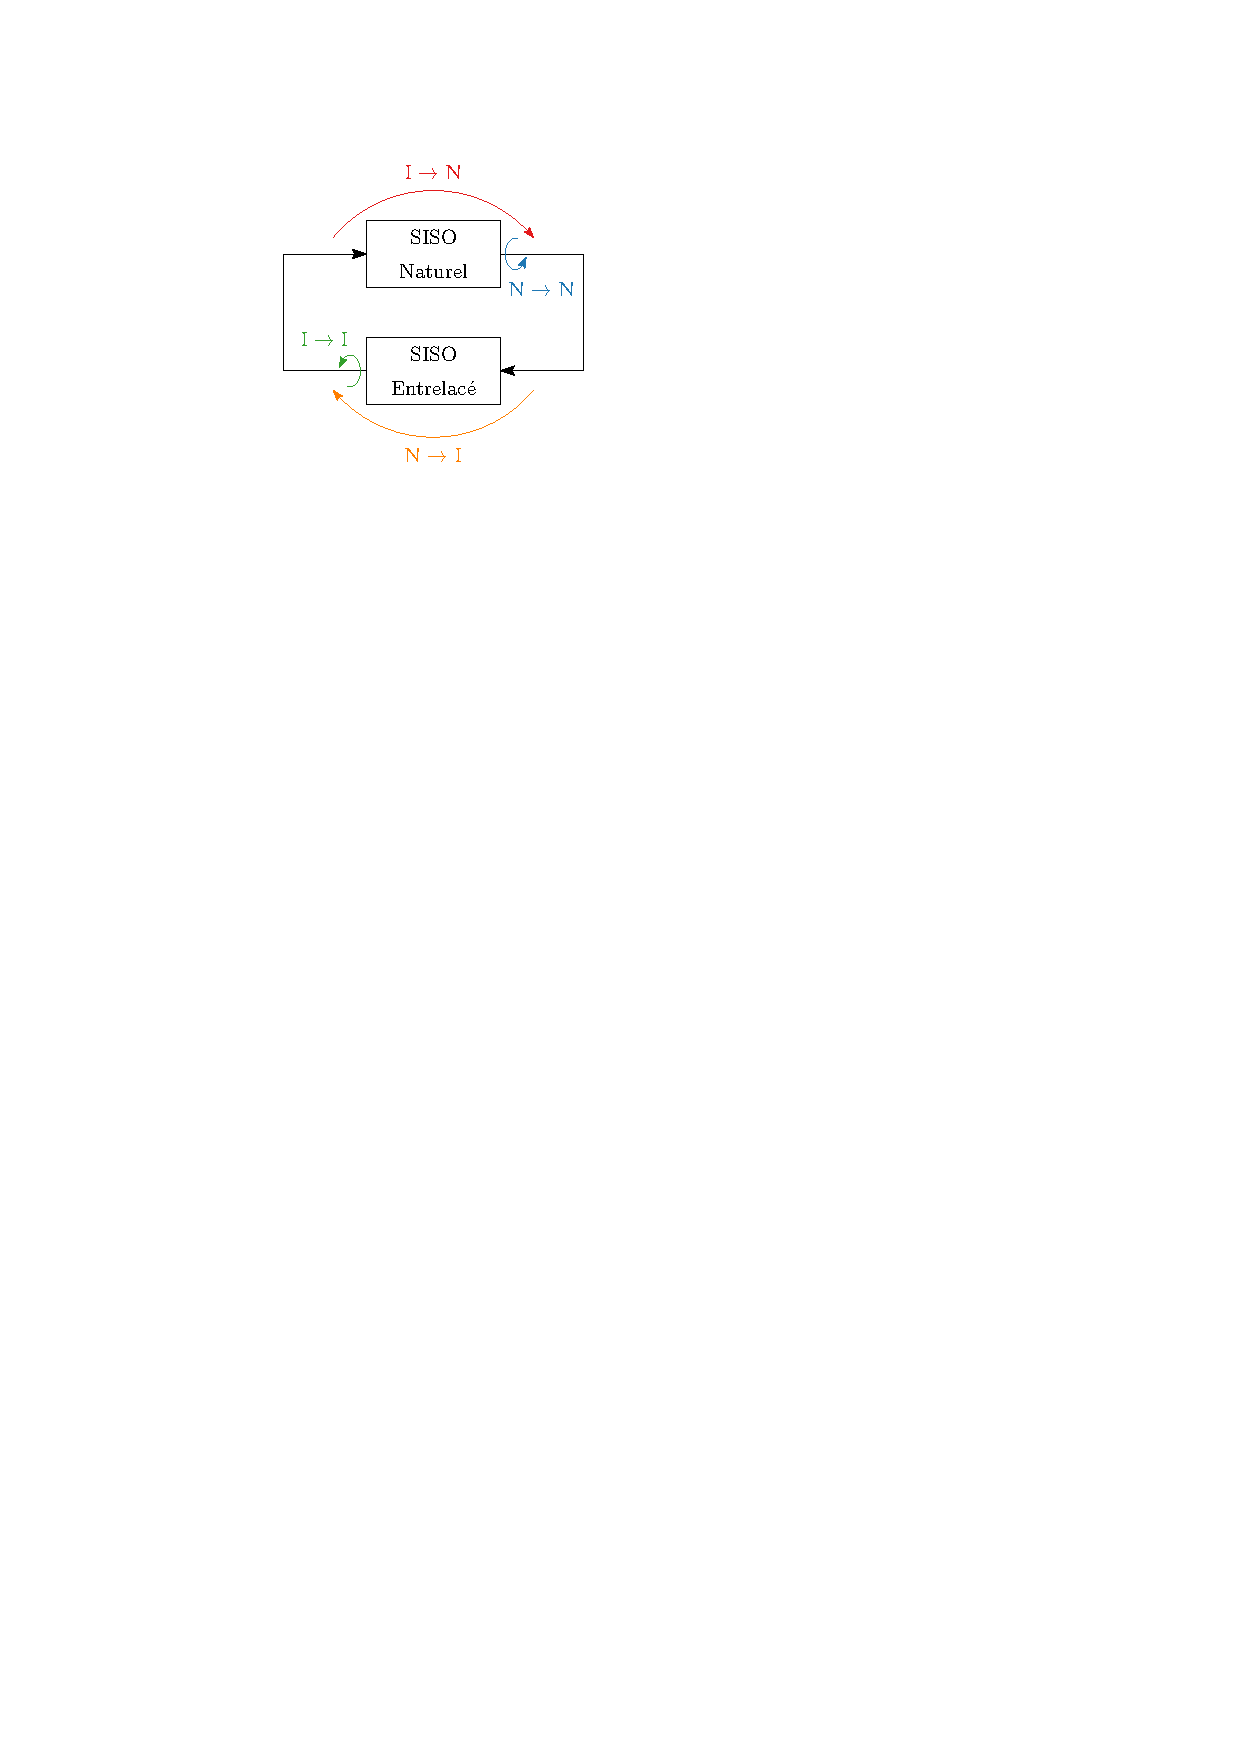
\includegraphics[width=7cm]{main/ch2_fig/ipe/osc.pdf}
	\caption{\label{fig:osc}Les différentes oscillations de l'information extrinsèque possibles.}
\end{figure}

Maintenant, ces statistiques sur le nombre d'oscillations vont être détaillées. D'abord dans le cas de standard LTE et 
ensuite, plus sommairement en raison de l'interprétation similaire des résultats dans le cadre du standard CCSDS. 
Plusieurs valeurs de SNR sont considérés afin d'analyser les oscillations suivant le contexte de fonctionnement du 
décodeur itératif (zones de non-convergence, de convergence et de plancher d'erreurs). Pour toutes ces statistiques, les 
trames considérées sont au nombre de 100. Tout d'abord l'étude sera statique : les moyennes et distribution des 
oscillations par bits seront présentés. Ensuite elle sera dynamique en considérant l'évolution des oscillations au cours 
des itérations.

\subsection{Standard LTE}
\subsubsection{Nombre moyen d'oscillations par bit}
La première statistique aisément obtenable est le nombre moyen d'oscillations par bits. Les bits peuvent être 
catégorisés selon deux groupes principaux :
\begin{itemize}
	\item bits appartenant à une trame corrigée à la dernière itération,
	\item bits appartenant à une trame erronée à la dernière itération.\newline
\end{itemize}
Ensuite, ce deuxième groupe peut lui-même être subdivisé :
\begin{itemize}
	\item bits corrects à la dernière itération dans un trame erronée à la dernière itération,
	\item bits erronés à la dernière itération dans un trame erronée à la dernière itération. \newline
\end{itemize}
La Figure \ref{ch2:fig:meanlte} présente l'évolution du nombre d'oscillations par bit selon la classification qui 
vient d'être introduite et ce, en fonction de la diminution du taux d'erreur trame pour le standard LTE. La sous-figure 
(a) correspond à la zone de non-convergence, les sous-figures (b) et (c) à la zone de convergence et finalement la (d) à 
la zone du plancher d'erreur. Plusieurs constations notables peuvent en être extraites. 

Tout d'abord, le nombre d'oscillations est le même que l'on considère comme référence le décodeur opérant dans le 
domaine naturel ou celui opérant le domaine entrelacé. Ainsi, dans la suite, uniquement les oscillations $N\rightarrow N$ 
et $N\rightarrow I$ seront considérées dans la suite des analyses.
Ensuite, quelque soit la valeur du SNR, les informations extrinsèques d'une trame corrigée n'oscillent pas ou très 
peu. En comparaison, les informations extrinsèques d'une trame erronée oscillent quant à elles environ dix fois plus.
Cette constatation est le principe fondamental des critères d'arrêts SCR et SDR. En effet, le nombre d'oscillations 
permet de savoir si une trame a convergé ou non.

\begin{figure}[tb]
	\begin{center}
	\includegraphics[]{main/ch2_fig/tikz/m_lte.pdf}
	\caption{Oscillations pour différents taux d'erreurs trame cibles, standard LTE \label{ch2:fig:meanlte}}
	\end{center}
\end{figure}

Toujours à partir de cette Figure, en considérant uniquement les trames erronées, il est visible que le nombre moyen 
d’oscillations par bits (tous bits confondus) est très proche du nombre moyen d’oscillations par bits corrigés. Ceci 
provient du fait que le nombre de bits erronés par trame erronée (BE/FE) est relativement faible. Ainsi, dans une trame 
erronée, pour les valeurs de SNR considérés la majorité des bits sont corrigés. Plus encore, dans la zone du plancher 
d'erreur le BE/FE est très faible (inférieur à la dizaine).

Il est encore plus remarquable que les bits erronés 
oscillent plus que les bits corrigés. Plus la valeur de SNR augmente, plus cette constatation est vraie. En effet, les 
bits erronées oscillent en moyenne environ dix fois pour l'oscillation $N\rightarrow N$ et environ 16 fois pour 
l'oscillation $N\rightarrow I$, ce quelque soit la valeur du SNR. En revanche, le nombre d'oscillations des bits corrigés 
diminue graduellement lorsque la valeur de SNR augmente. Ainsi, au sein des trames erronées, dans le plancher d'erreur 
du standard LTE, les bits erronés oscillent quatre fois plus que les bits erronés.

Ainsi, pour conclure, les observations liées à cette Figure, pour une raison de symétrie dans l'architecture du décodeur 
le nombre d'oscillations par bit est lui aussi symétrique vis-à-vis de l'entrelaceur. Ainsi, uniquement deux 
oscillations peuvent être considérées. Permettant les critères d'arrêts SDR et SCR, le nombre d’oscillation par bit est 
un critère discriminant les trames corrigées. Finalement, si un bit est erroné, alors, en moyenne, il aura plus oscillé 
que les bits corrigés. Afin de pouvoir améliorer le décodage, il est intéressant d'essayer d'établir si la réciproque : 
\og Un bit ayant oscillé plus que la moyenne des oscillations est-il erroné ? \fg Or, pour ceci, ces statistiques doivent
être présentées selon une granularité différente.

\subsubsection{Nombre d'oscillations par trame en fonction des itérations} 
Dans cette partie, les oscillations sont présentées au cours des itérations. Uniquement deux valeurs de SNR sont 
considérées afin de faciliter l'analyse. La première correspond à un taux d'erreur trame de $10^{-2}$, donc au début de 
la zone de convergence et est présenté en Figure \ref{ch2:fig:it_lte_1}.

\begin{figure}[!tb]
	\hspace*{-.7cm}
	\includegraphics[]{main/ch2_fig/tikz/it_lte10-2.pdf}
	\caption{Oscillations au cours des itérations dans le cadre du standard LTE pour un taux d'erreur trame de $10^{-2}$ \label{ch2:fig:it_lte_1}}
\end{figure}

Cette Figure est divisée en six sous-figures. La première colonne traite des trames erronées à l'issue du processus 
itératif. La seconde colonne concerne les trames corrigées. Trois quantités sont présentées : le nombre d'oscillations 
$N\rightarrow N$, le nombre d'oscillations $N\rightarrow I$ et le nombre d'erreurs.

Nous pouvons remarquer que les trames corrigées à la 32\textsuperscript{ème} itération non corrigées à l'issue de la 
10\textsuperscript{ème} itération sont marginales. Ceci est à corroborer avec le choix réalisé dans la majorité des 
architectures de turbo décodeur de fixer le nombre maximal d'itérations à moins de 10.
Il est aussi remarquable que le nombre d'erreurs semble être fortement corrélé avec le nombre d'oscillations. En effet, 
les rares trames erronées n'oscillant que peu sont celles qui ne possèdent que peu d'erreur. Plus généralement,
le nombre d'oscillations semble correspondre au double du nombre d'erreurs.

La Figure \ref{ch2:fig:it_lte_2} présente les mêmes donnés que la Figure \ref{ch2:fig:it_lte_1} mais les résultats sont
obtenus pour un taux d'erreur trame cible de $10^{-5}$. Pour le standard LTE, ceci correspond à un fonctionnement du 
turbo décodeur au début du plancher d'erreur. Nous pouvons remarquer que pour les trames corrigées, la convergence vers 
la bonne solution est plus rapide : uniquement quelques itérations sont nécessaires. Pour les trames erronées à l'issue 
du processus itératif, des trames possédant un nombre important d'erreurs sont rares. Elles correspondent à celles 
présentant le plus grand nombre d'oscillations. De fait, la majorité des trames erronées possèdent un faible nombre 
d'erreurs, qui reste majoritairement constant après la cinquième itération.

Finalement, ces nouvelles observations permettent d'observer les oscillations en fonction des itérations. Il est alors 
observable que d'une part, pour les trames erronées, deux \og modes \fg d'oscillations sont visibles :
\begin{itemize}
	\item le nombre d'oscillations est très important, subi des variations au cours des oscillations mais reste dans la plage de valeurs $[200,400]$.
	\item le nombre d'oscillations est faible et subi peu de variations.
\end{itemize}

D'autre part, il a été noté une corrélation forte entre nombre d'erreurs et nombre d'oscillations. Cependant, ces 
observations sont réalisés au niveau trame. Il est donc maintenant nécessaire de descendre en granularité pour observer 
la distribution des oscillations dans les trames erronées.

\begin{figure}[!hb]
	\hspace*{-.7cm}
	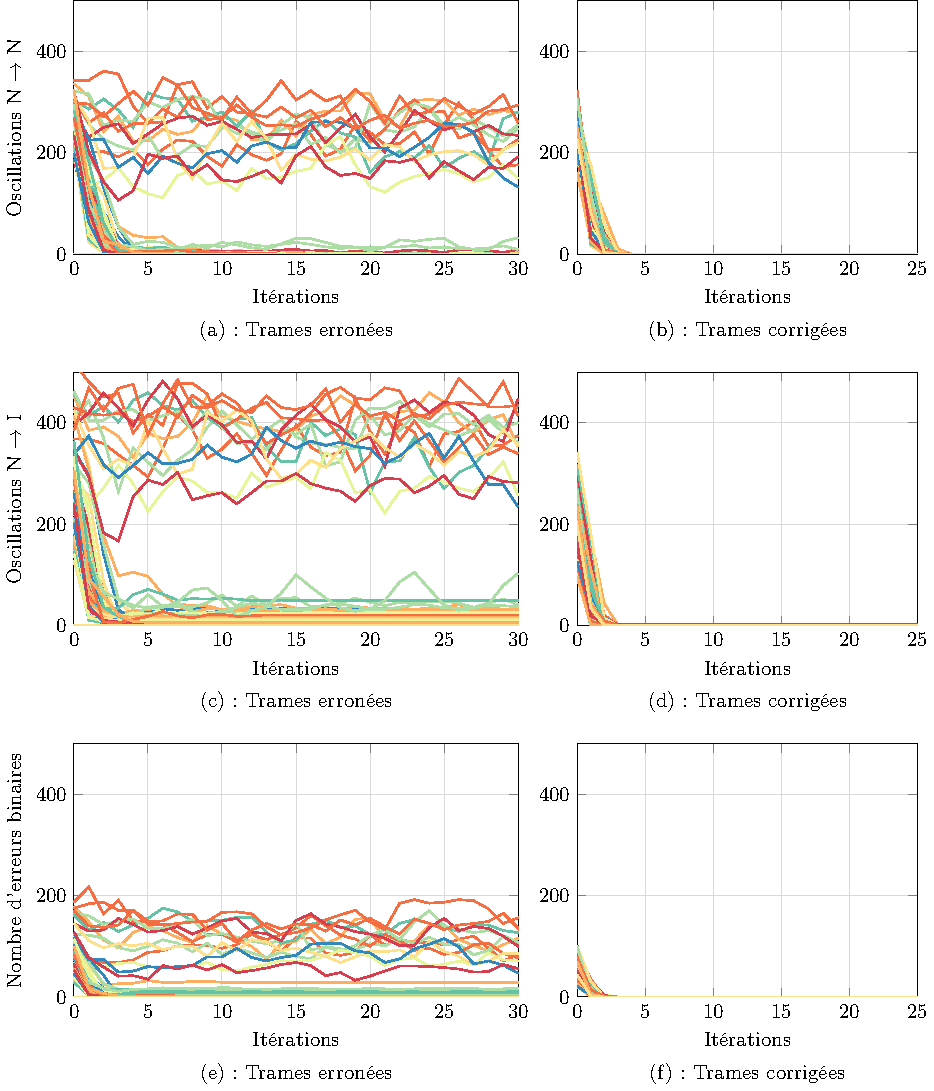
\includegraphics[]{main/ch2_fig/tikz/it_lte10-5.pdf}
	\caption{Oscillations au cours des itérations dans le cadre du standard LTE pour un taux d'erreur trame de $10^{-2}$ 
	\label{ch2:fig:it_lte_2}}
\end{figure}

\subsubsection{Distributions du nombre d'oscillations pour les trames erronées} 
Dans cette section, la distribution des oscillations dans les trames erronées est analysé. Dans les sections précédentes,
il a été montré que les bits erronées d'un trame erronée oscillent plus que les bits corrects. Les données présentées 
maintenant permettent d'établir si la réciproque est vraie. 
Pour ce faire, la Figure \ref{fig:d_lte_10-2} présente l’occurrence du nombre d'oscillations par bit pour un taux 
d'erreur trame cible de $10^{-2}$. Cette Figure, en deux parties, considère d'abord les oscillations $N\rightarrow N$ et 
$I\rightarrow I$ (a) puis, les oscillations $N\rightarrow I$ et $I\rightarrow N$ (b). Les occurrences sont normalisées 
par rapport au nombre de bit total.

%À nouveau, le comportement des oscillations est semblable vis-à-vis de la référence (c'est-à-dire que l'on considère 
%$N\rightarrow N$ ou $I\rightarrow I$). 

Selon la Figure \ref{fig:d_lte_ni_-2} (a), $20\%$ des bits sont corrects et n'ont pas oscillé. Il est remarquable que 
les nombres d'oscillations impairs sont sous représentés vis-à-vis des pairs. Il semblerait donc que, majoritairement, 
la première décision prise par un SISO soit la bonne. Néanmoins, nous n'avons pu tirer d'analyse plus conséquente de 
cette observation. La distribution des oscillations des bits erroné et relativement équirépartie. 

Les oscillations $N\rightarrow I$ et $I\rightarrow N$ ne présentent pas d’irrégularité comme constatée dans les cas 
$N\rightarrow N$ et $I\rightarrow I$. L'allure de la distribution des oscillations pour les bits corrects à l'issu du 
processus itératif semble être la composition de deux gaussiennes, l'une centrée en $0$ et l'autre en $14$. Pour les 
bits erronés, l'allure des distributions est aussi en forme de gaussienne et centrée autour de $16$.

Pour le taux d'erreur trame considéré pour cette Figure, le nombre moyen de bit erroné par trame erroné (BE/FE) vaut 
113. Cela signifie (en considérant la taille de la trame) que $11\%$ des bits sont erronées dans une trame erronée. 
Si le nombre d'oscillations est pris en considération, alors la probabilité de bit erroné varie de $0,1\%$ à $19,9\%$. 
Pour les bits oscillant moins de 11 fois, cette probabilité est inférieure à la probabilité moyenne. Par contre, elle
est supérieure à la probabilité moyenne si le bit considéré à oscillé 11 fois ou moins. Ainsi, en considérant les bits 
ayant oscillé 15 fois ou plus, la probabilité que ces bits vaut $18\%$. Ainsi, la probabilité de tirer un bit erroné à 
doublé. Néanmoins, les bits erronés oscillent eux aussi. De plus, comme ils sont majoritaires, les 

\begin{figure}[!hb]
	\centering
	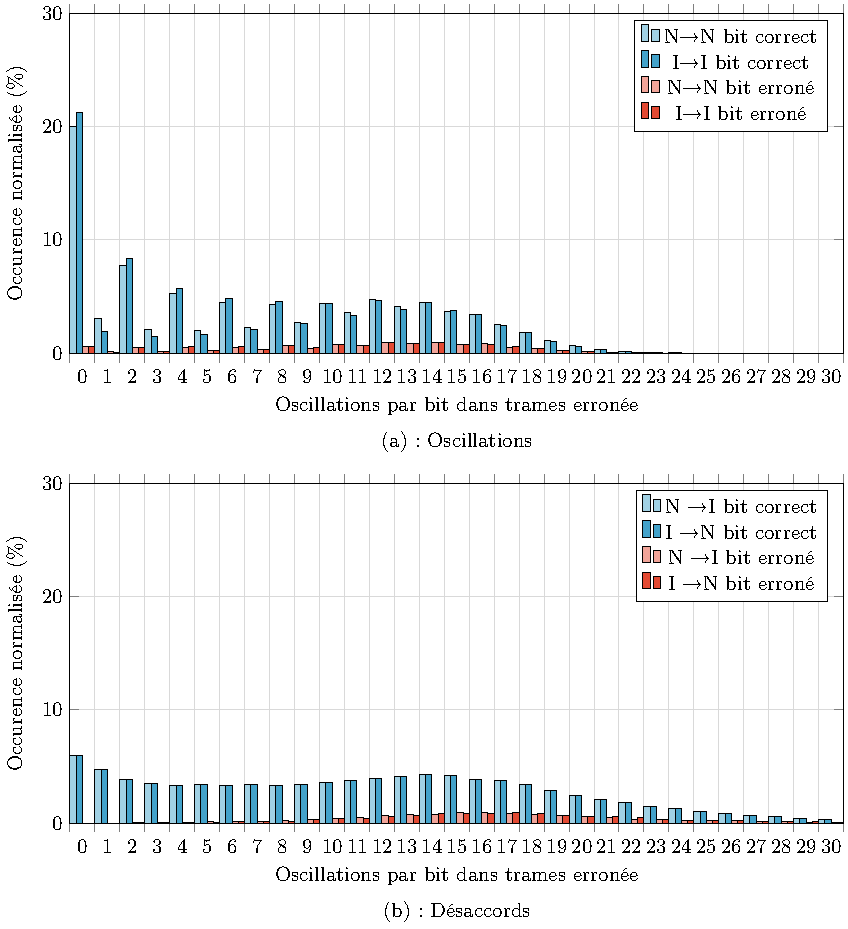
\includegraphics[]{main/ch2_fig/tikz/d_lte_10-2.pdf}
	\caption{Distribution du nombre d'oscillations par bit pour un taux d'erreur trame de $10^{-2}$, pour le standard LTE \label{fig:d_lte_10-2}}
\end{figure}
